\chapter{Proteome Profiling}
\label{chap:protprof}

The Proteome Profiling modules is designed to identify differentially expressed
protein under various experimental conditions. A typical example is to compare the
effect of two substance over protein expression using whole cell lysates.

\section{Definitions}

Before explaining in detail the interface of the module and how does the module work, 
let's make clear the meaning of some terms that will be used in the following paragraphs.

\phantomsection
\begin{itemize}
    \item \textit{Detected protein}: any protein detected in any of the mass spectrometry
    experiments including the control experiments.
    \item \textit{Relevant proteins}: a detected protein with a Score value above
    a user-defined thresholds (page \pageref{par:protprofScoreValue}).
\end{itemize}

\section{The input files}

The Proteome Profiling module requires only one input file. This Data file must follow
the guidelines specified in \autoref{sec:dataFile}. In short, the Data file must
have a tabular format with tab separated columns and the name of the columns are
expected as first row. All columns given as input in section Column numbers of Region
Configuration Options of the interface (\autoref{fig:protprofTab}) must be present
in the Data file.

\section{The interface}

The tab of the Proteome Profiling module is divided in two regions (\autoref{fig:protprofTab}).

\begin{figure}[h]
    \centering
    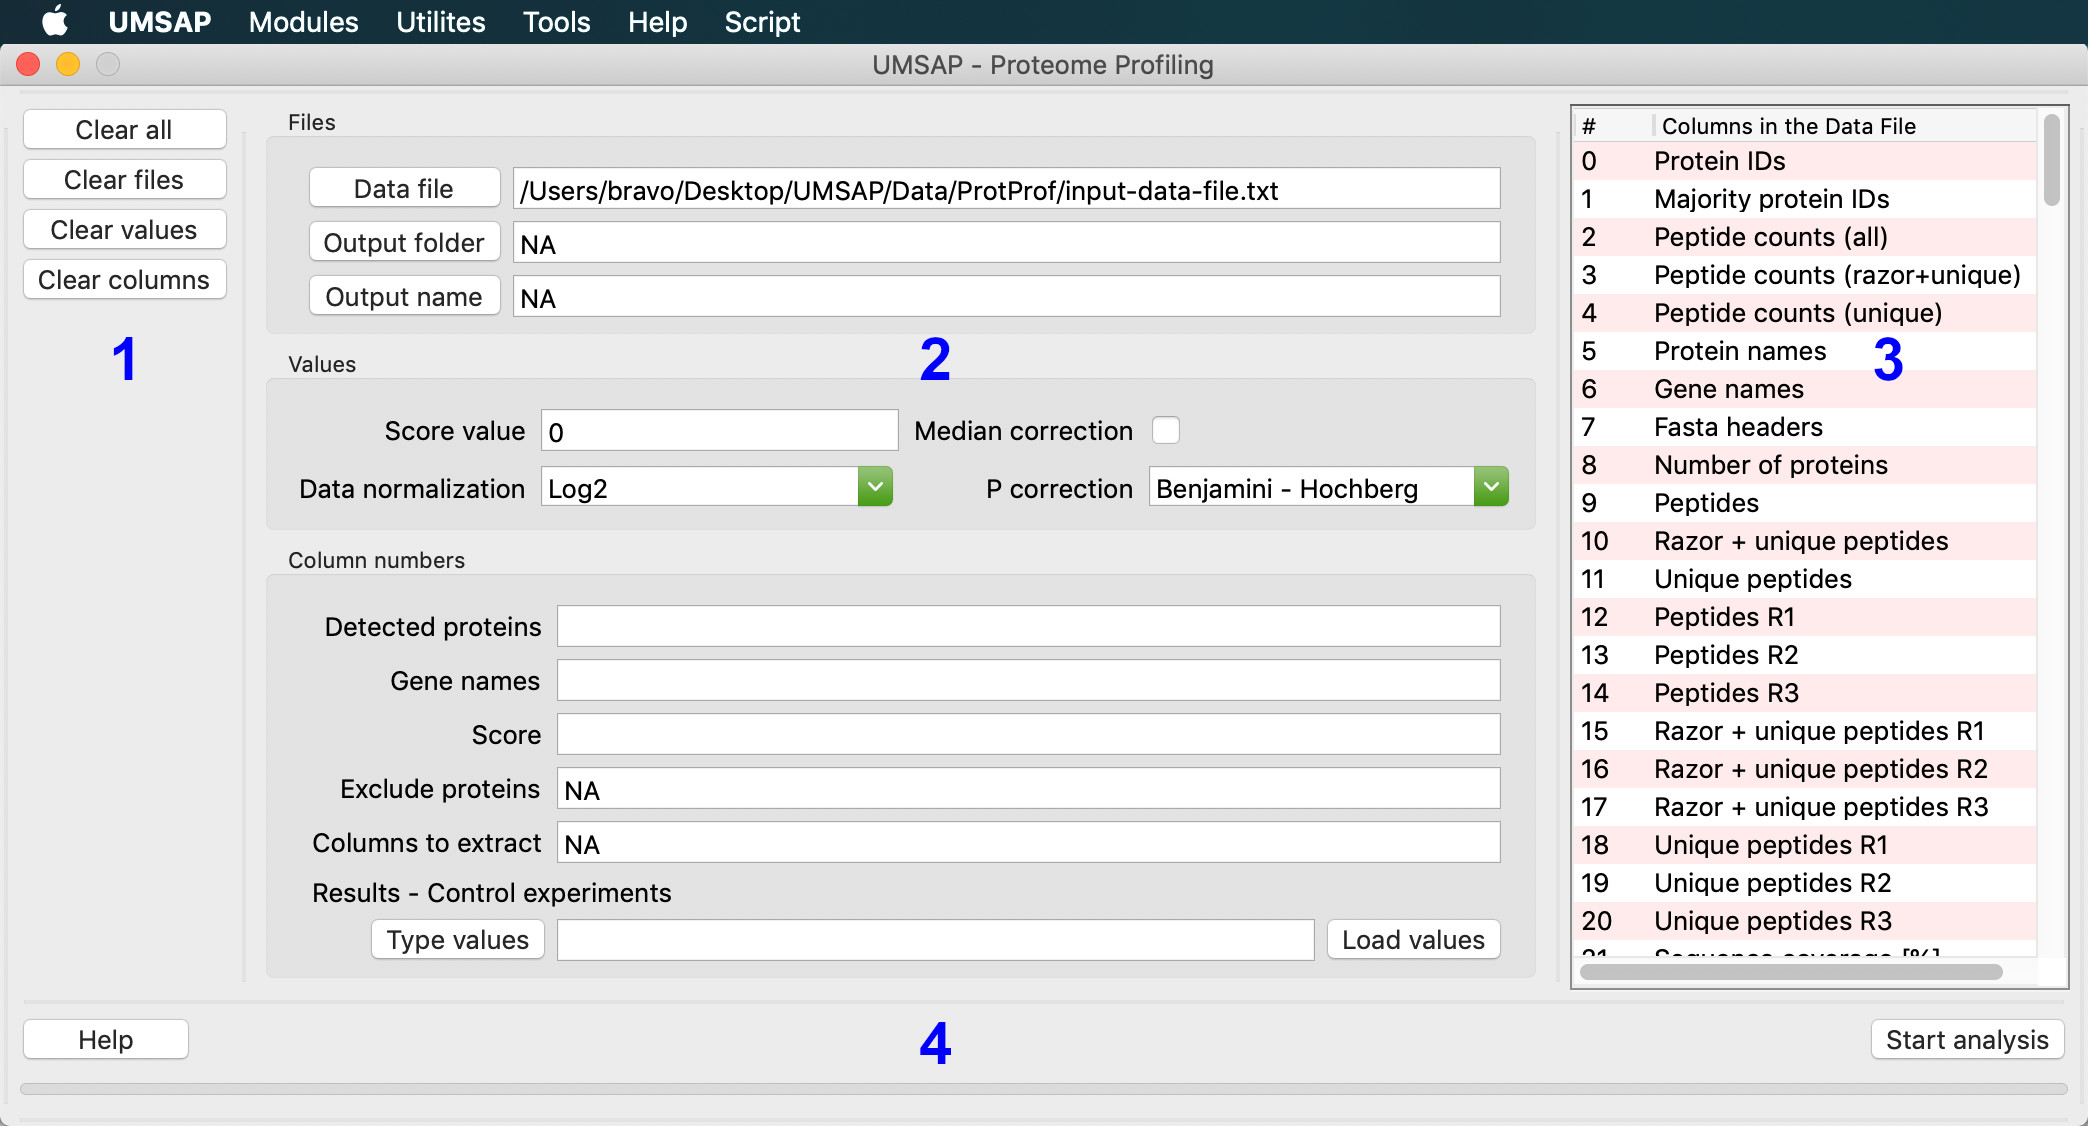
\includegraphics[width=0.7\textwidth]{./IMAGES/MOD-PROTPROF/protprof-mod.jpg}
    \caption[The Proteome Profiling module tab]{\textbf{The Proteome Profiling module
    tab.} This tab allows users to perform a proteome profiling analysis.}
    \label{fig:protprofTab}
    \vspace{-5pt}
\end{figure}

The Data File Content region holds only a table to show the name of the columns in
the selected Data File. The table will be automatically filled after selecting the
file. Selected rows in the table can be copied (Cmd+C) and pasted (Cmd+V) to the
text fields in region Configuration Options.

The Configuration Options region contains all the fields needed to configure and
run the analysis.

Section Files contains two buttons and a text field. Here users select the input
and output files for the analysis.

\num{1}. The button UMSAP allows users to browse the file system to select the location
and name of the .umsap file. When selecting an already existing .umsap file the operating
system will ask if it is ok to replace the file, the answer can be yes since UMSAP
will never overwrite or replace an .umsap file, instead the new analysis will be
added to the already existing file. Only .umsap files can be selected here.

\num{2}. The button Data allows users to browse the file system to select the input
data file that will be used for the analysis. The Data file is expected to be a
plain text file with tab separated columns and the name of the columns in the first
row of the file. In addition, columns to be analyzed must contain only numbers and
must be of the same length. Only .txt files can be selected here.

\num{3}. The text field Analysis ID allows users to provide an ID for the analysis
to be run. The date and time of the analysis will be automatically added to the
beginning of the name.

Section Data Preparation contains four dropdown boxes. Here users select how the data
in the Data file should be prepared before starting the analysis.

\num{1}. The dropdown Treat \num{0}s as missing values allows user to define how
to handle \num{0} values present in the Data file.

\num{2}. The dropdown Transformation allows user to select the Transformation method
to be applied to the data.

\num{3}. The dropdown Normalization allows users to select the Normalization method
to be applied to the data.

\num{4}. The dropdown Imputation allows user to select the Imputation method used
to replace missing values in the data.

Section User-defined values contains two text fields and three dropdown box. Here
users configure the Proteome Profiling analysis to be run.

\phantomsection
\num{1}. The text field Score Value\label{par:protprofScoreValue} allows users to
define a threshold value above which the detected proteins will be considered as
relevant. The Score value is an indicator of how reliable was the detection of
the protein during the MS experiments. The value given to UMSAP depends on the program
generating the Data file. Only one real number equal or greater than zero will be
accepted as a valid input here. A value of zero means all detected proteins will be
treated as relevant proteins.

\num{2}. The dropdown Samples allows users to specify whether samples are independent
or paired. For example, samples are paired when the same Petri dish is used for the
control and experiments.

\num{3}. The text field $\alpha$ level allows users to define the significance level
used for the analysis. Only a number between \num{0} and \num{1} will be accepted
here.

\num{4}. The dropdown Intensities allows user to specify whether the intensity values
in the Data file represent absolute or a ratio of intensities.

\num{5}. The dropdown P Correction allows user to select the correction method for
the p values calculated during the analysis.

Section Column numbers contains five text fields. Here, users provide the column
numbers in the Data file from where UMSAP will get the information needed to perform
the analysis of the module. All columns specified in this section must be present
in the Data file. Column numbers start at \num{0}. The column numbers are shown in
the table of Region Data File Content after the Data file is selected.

\num{1}. The text field Detected Proteins allows users to specify the column in
the Data file containing the protein identifiers found in the Data file. Only one
integer number equal or greater than zero will be accepted here. 

\num{2}. The text field Gene Names allows users to specify the column in the Data
file containing the gene names of the proteins found during the MS experiments.
Only one integer number equal or greater than zero will be accepted here. 

\num{3}. The text field Score allows users to specify the column in the Data file
containing the Score values. It is in this column where the program will look for
the values to be compared against the Score threshold given in section User-defined
values. Only one integer number equal or greater than zero will be accepted here. 

\num{4}. The text field Exclude proteins allows users to specify several columns
in the Data file. Proteins found in these columns will be excluded form the analysis.
The module assumes that these columns contains numeric values and values greater
than zero indicate that the respective protein must be eliminated from the analysis.
Only integer numbers equal or greater than zero will be accepted here. If left empty
all proteins will be considered during the analysis. 

\num{5}. \label{par:protprofResultControl} The text field Results - Control experiments
allows users to specify the columns in the Data file containing the results of the
experiments. The button Type Values calls a helper window (\autoref{fig:protprofResControlWindow})
where users can type the information needed. Duplicate column numbers are not allowed here.

\begin{figure}[h]
    \centering
    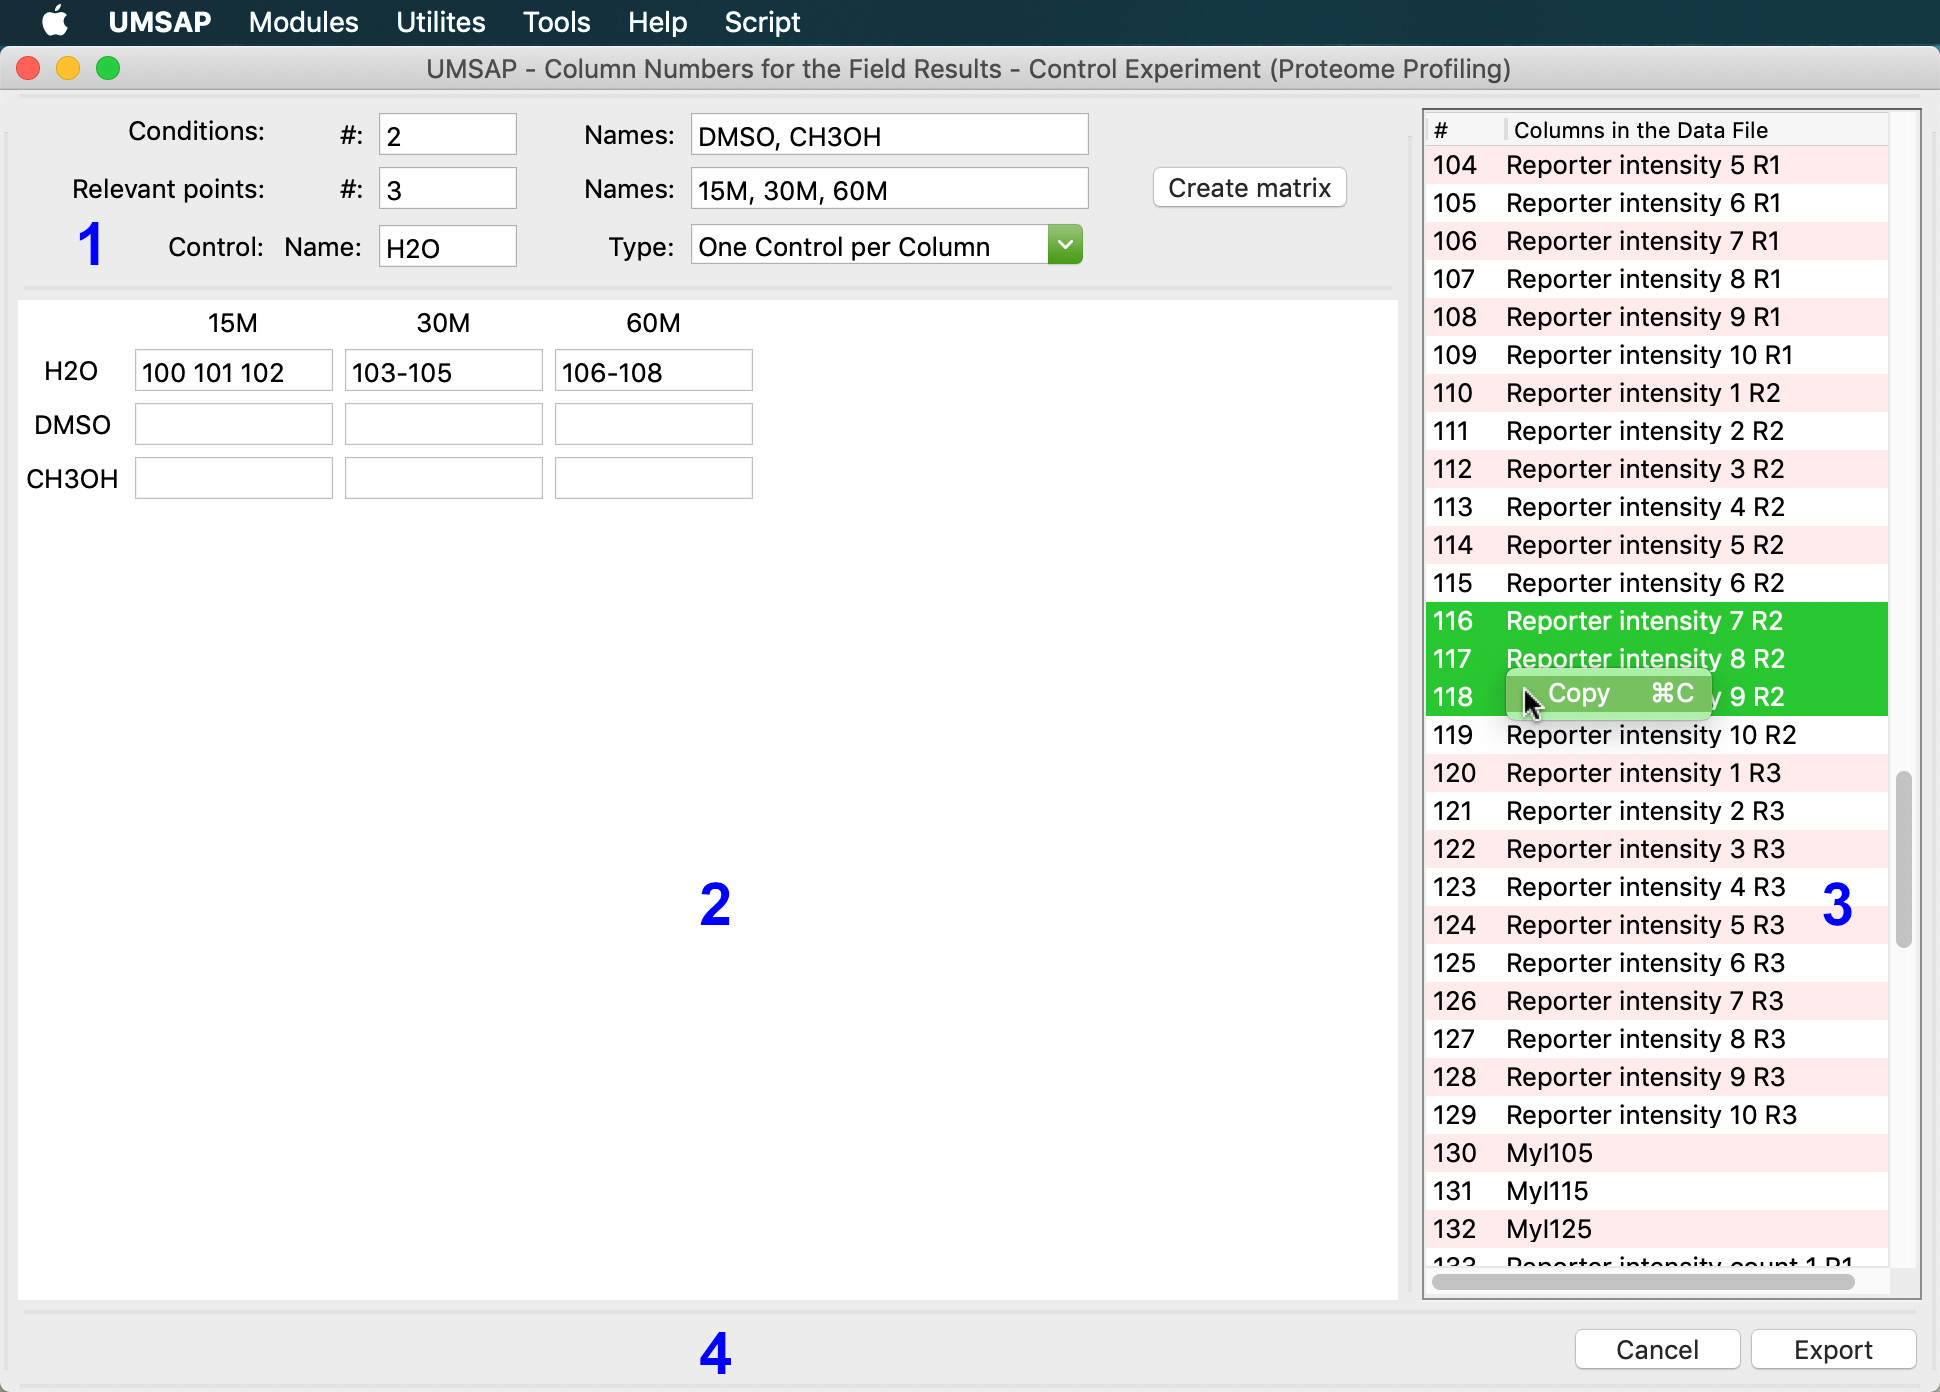
\includegraphics[width=0.7\textwidth]{./IMAGES/MOD-PROTPROF/protprof-rescontrol.jpg}
    \caption[The Result - Control experiments helper window for the Proteome Profiling module]{\textbf{The Result - Control experiments helper window for the Proteome Profiling module.} This window allows users to specify the column numbers in the Data file containing the MS results for the selected conditions, relevant points and control experiments.} 
    \label{fig:protprofResControlWindow}
    \vspace{-5pt} 	
\end{figure}

The helper window is divided in two Regions. Region Data File Content will show the 
column numbers and names of the columns present in the selected Data file. Region
Configuration Options has two sections. The upper section allows defining the number
of conditions and relevant points analyzed, to define the kind of control experiment
used as well as the label for conditions, relevant points and control experiment.
The button Setup Fields allows creating the matrix of text fields in the bottom section
where users type the column numbers. Each text field should contain the column
numbers with the MS results for the given experiment. The values for the text fields
should be positive integer numbers or a range of integers, e.g. 
\numrange[range-phrase=--]{60}{62} or left blank. Selected rows in the table can
be copied (Cmd+C) and then pasted (Cmd+V) in the text fields. Duplicate column numbers
are not allowed. 

\section{The analysis}
\label{sec:protprofTTest}

First, UMSAP will check the validity of the user-provided input and then the selected
Data file is read. The columns specified in section Column numbers are extracted
from the Data file. All other columns present in the Data file are discarded. After
this, all steps selected in the Data Preparation section are applied to the columns
specified in the text field Result - Control experiments (\autoref{chap:dataPrep}).
Then, the following actions are performed.

All proteins found in the Exclude proteins columns are discarded. Also, all proteins
with a Score value lower than the defined threshold are removed. The resulting data
is used for the proteome profiling analysis \cite{Aguilan2020}. This includes the
calculation of the fold change (FC) (\autoref{eq:protprofFC}), the p values and the correction
of the p values. Currently, the p values are calculated using a t-test.

\begin{equation}
\label{eq:protprofFC}
FC = ave(I_{C, RP}) / ave(I_{Control})
\end{equation}

\section{The result window}

The window showing the results from a Proteome Profiling analysis is divided in three
regions (\autoref{fig:limprotResWindow}).

\begin{figure}[h]
    \centering
    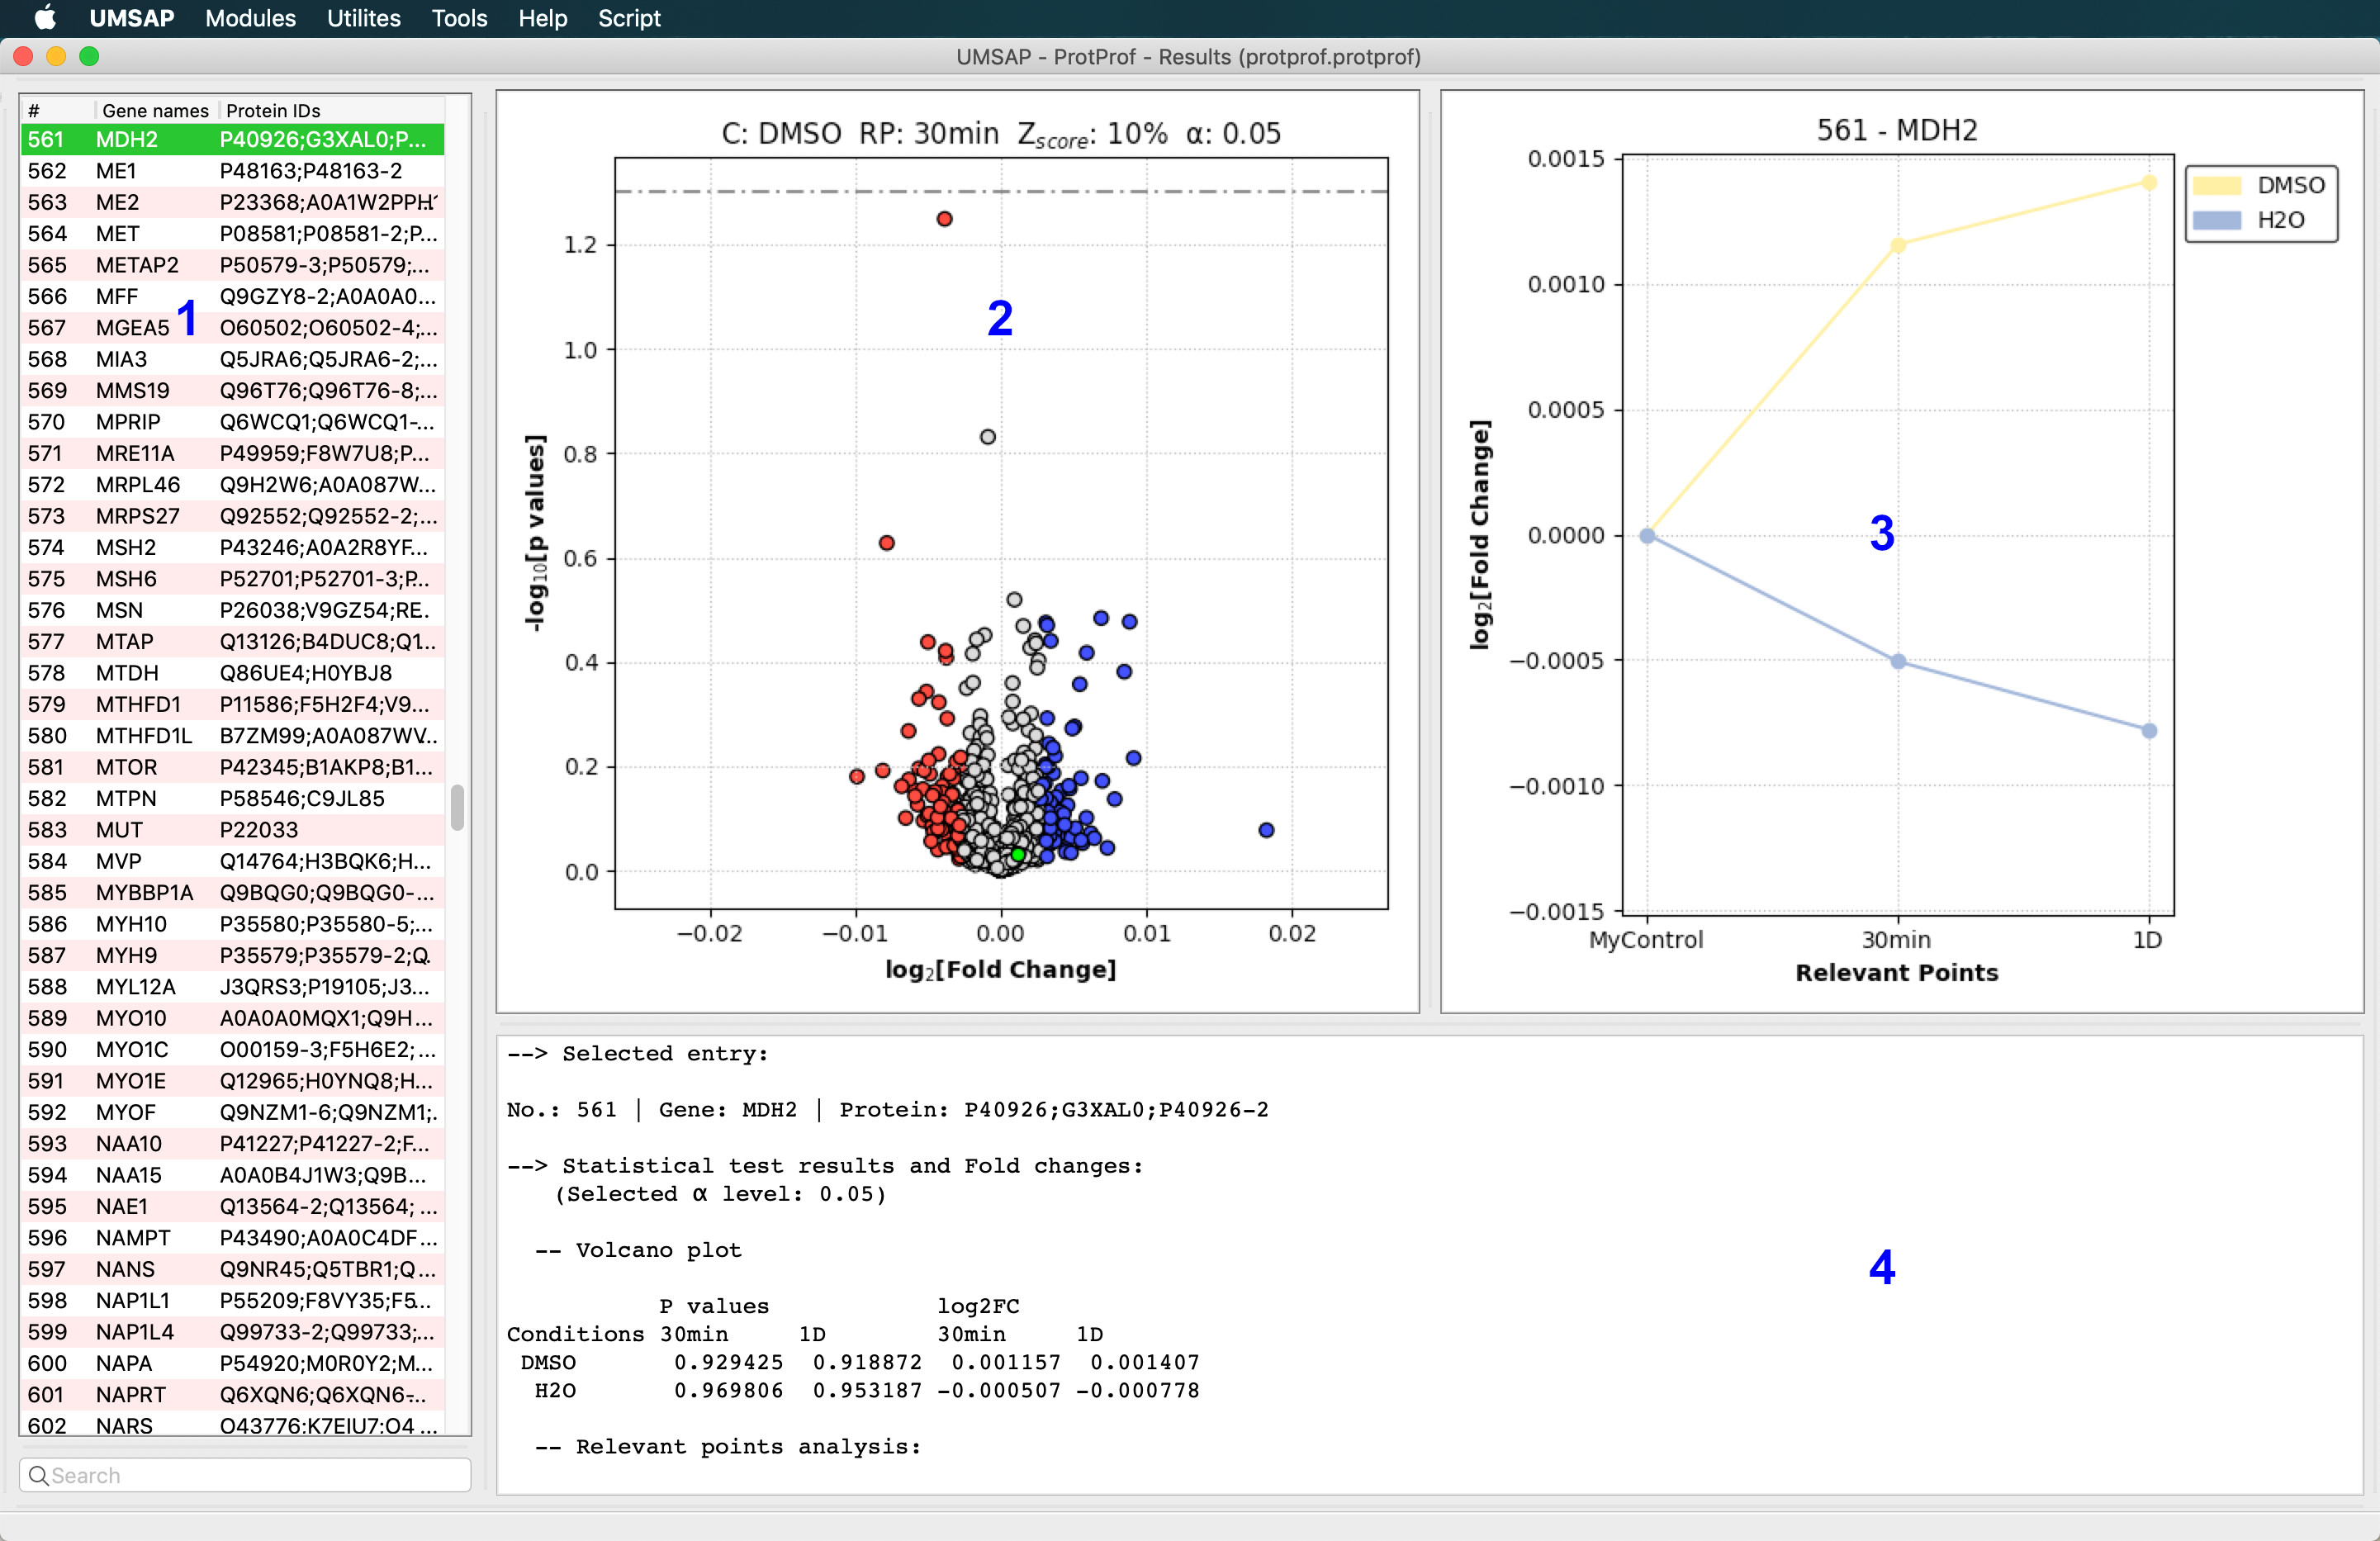
\includegraphics[width=0.8\textwidth]{./IMAGES/MOD-PROTPROF/protprof-frag.jpg}
    \caption[The Proteome Profiling result window]{\textbf{The Proteome Profiling
    result window.} Users can perform here the analysis of the proteome profiling
    results.} 
    \label{fig:protprofResultsWindow}
    \vspace{-5pt} 	
\end{figure}

Region Protein List contains a table with the protein IDs and Gene names that were not
excluded from the analysis and whose Score values are greater than the user-defined
threshold. Selecting a protein in the table will highlight the protein with a green
dot in the Volcano plot and display the $log_2[FC]$ evolution along the relevant points
in region Plots. In addition, information about the selected protein will be displayed
in Regions Profiling details.

Region Plots contains two plots. A volcano plot showing the results for the t-test
comparing the condition (C), relevant point (RP) to the corresponding control. The
points in the plot can be colored by Z-score allowing to quickly identified the top
up (blue) or down (red) regulated proteins or according to the hyperbolic curve cut-off
\cite{LI2012}. Selecting a protein in the plot will highlight the selected protein
in region Protein List and display information about it in region Profiling details,
or it will add a label to the plot.

The plot of $log_2[FC]$ vs Relevant points allows to see the evolution of the FC
along the Relevant points and to compare the FC across the various conditions in
the analysis. The error bars in the plot represent the confident interval for the
FC values calculate at the $1-\alpha$ level. The gray zone shown in the plot represent
the maximum and minimum FC value for each Relevant point across all Conditions in
the analysis.

Region Profiling details shows a summary of the results for the selected protein.
Proteins can be selected in the table in region Protein List or in the volcano plot
of region Plots. The information includes the calculated p and $log_2[FC]$ values
as well as averages and standard deviations for intensities and ratios.

\section{The Tools menu}
\label{sec:protprofTools}

The Tools menu in the window showing the results from a Proteome Proteolysis analysis
allows user to display any of the analyses contained in the selected .umsap file.

The submenu Volcano Plot allows to control the appearance of the volcano plot. Users
can change the the Condition - Relevant point displayed, add labels (Shift+A) to
the points in the plot, toggle between using the left click of the mouse for selecting
proteins or adding labels (Shift+P), adjusting the Color Scheme of the plot, show
corrected p values, create an image of the plot (Shift+I) or reset the zoom level of
the plot (Shift+Z). The entry Color Scheme allows coloring points in the Volcano plot
by Z-score or the hyperbolic curve cut-off. It also allows configuring the Z-score
threshold and the hyperbolic curve parameters.

The submenu FC Evolution allows toggling the display of the maximum/minimum area,
to create an image of the plot (Alt+I) and to reset the zoom level of the plot (Alt+Z).

The submenu Lock Plot Scale allows setting the scale of the plot. If this option
is set to No, then the scale of the plot is allowed to change every time the plots
are updated, for example changing the Condition - Relevant point displayed for a
given analysis. If set to Date, then the scale of the plot is fixed for all Conditions
- Relevant points in one analysis and updated every time a new analysis is displayed.
If set to Project, then all plots for all analysis will have the same scale.

The submenu Clear Selection allows removing any selection done by the user. In
particular, the entry All (Cmd+K) will remove all selections basically resetting
the state of the window.

The Tools menu also allows duplicating the window (Cmd+D) for easier comparison of
two or more analysis, checking the Data Preparation steps of the analysis (Cmd+P),
and exporting the results of the analysis to a tab separated CSV file (Cmd+E).

\newpage
\subsection{Filters}

The proteins displayed in the Volcano plot can be filtered in order to display only
proteins with a particular behavior. The submenu Filters allows managing which 
proteins will be displayed. Filters are applied to the current Condition and Relevant
point shown in the Volcano plot. If the Condition or the Relevant point shown is
changed, the new plot will show the proteins obtained after the filter was applied.
This allows to follow the behavior of the filtered proteins in all Conditions and
Relevant points. Any number of filters can be applied. The applied filters are shown
in the bottom left corner of the window. Selecting a different analysis will reset
the filters unless the option Auto Apply (Shift+Cmd+F) is selected. Also, filters
can be manually reapplied with the menu entry Apply All (Shift+Cmd+A). Filter can
also be removed, copied (Shift+Cmd+C) and pasted (Shift+Cmd+V) in a different window
and saved (Shift+Cmd+S) and load (Shift+Cmd+L) from/to the .umsap file.

Currently, the implemented filters are:

\textbf{\textit{\underline{FC Evolution}}}

This filter allows identifying proteins whose FC evolution follows a defined pattern.
For example, all proteins for which the FC is always greater than \num{0} or proteins
that show $FC > 0$ in one condition but $FC < 0$ in others. The filter can be applied
to the current selected Condition - Relevant point or considering any or all the
conditions.

\textbf{\textit{\underline{Hyperbolic Curve}}}

This filter allows identifying proteins above the Hyperbolic curve cut-off. It is
only applied to the current Condition - Relevant point.

\textbf{\textit{\underline{Log2FC}}}

This filter allows identifying proteins whose $log_2[FC]$ are greater or smaller
than the given value. It is only applied to the current Condition - Relevant point.

\textbf{\textit{\underline{P value}}}

This filter allows identifying proteins by the calculated p value. The p value
can be given in the 0 to 1 range or as a $-log10$ value. Regular or corrected P
values can be used in the filter. It is only applied to the current Condition -
Relevant point.

\textbf{\textit{\underline{Z score}}}

This filter allows identifying proteins by the Z score value of the FC. This is a
quick way to identify, for example, the top \SI{10}{\percent} up and down regulated
proteins. It is only applied to the current Condition - Relevant point.


































